\documentclass{standalone}
\usepackage{tikz,pgfplots,calc,tkz-euclide}
\usetikzlibrary{positioning,calc}
\usetikzlibrary{arrows}
\usepackage{tkz-euclide}
\usetkzobj{all}


\begin{document}
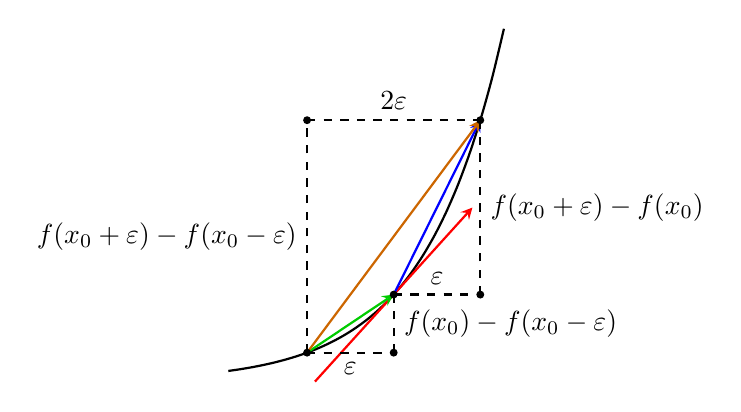
\begin{tikzpicture}[>=stealth, thick]
    \def\a{1}
    \draw[domain=-2:1.5,smooth,variable=\x,black] plot ({\x},{exp(\a*\x)});      
    \foreach \xx in {.1}{
        \draw[->, red, thick, domain=(\xx-1):(\xx+1),smooth,variable=\x] plot ({\x},{(\a*exp(\a*\xx))*(\x - \xx) + exp(\a*\xx)});      
    }


    \def\x{.1}
    \def\xp{1.2}
    \def\xm{-1}
    \def\y{{exp(\a*\x)}}
    \def\yp{{exp(\a*\xp)}}
    \def\ym{{exp(\a*\xm)}}

    \draw [->, green!80!black] (\xm, \ym) -- (\x, \y);
    \draw [->, blue] (\x, \y) -- (\xp, \yp);
    \draw [->, orange!80!black] (\xm, \ym) -- (\xp, \yp);

    \draw [dashed] (\xm, \ym) -- node[below] {$\varepsilon$} (\x, \ym);
    \draw [dashed] (\x, \y) -- node[above] {$\varepsilon$} (\xp, \y);
    \draw [dashed] (\x, \ym) -- node[right]{$f(x_0) - f(x_0 - \varepsilon)$} (\x, \y);
    \draw [dashed] (\xp, \y) -- node[right]{$f(x_0 + \varepsilon) - f(x_0)$} (\xp, \yp);


    \draw [dashed] (\xm, \ym) -- node[left]{$f(x_0 + \varepsilon) - f(x_0 - \varepsilon)$} (\xm, \yp);
    \draw [dashed] (\xm, \yp) -- node[above]{$2\varepsilon$} (\xp, \yp);

    \draw [fill = black, draw = black] (\x, \y ) circle (1pt);
    \draw [fill = black, draw = black] (\xp, \yp) circle (1pt);
    \draw [fill = black, draw = black] (\xm, \ym) circle (1pt);
    \draw [fill = black, draw = black] (\x, \ym) circle (1pt);
    \draw [fill = black, draw = black] (\xm, \yp) circle (1pt);
    \draw [fill = black, draw = black] (\xp, \y) circle (1pt);

\end{tikzpicture}
\end{document}